\chapter{Completed Work}


This work was published at Physical Review A \cite{de_leeuw_diffusion_2012},
and reprinted here in \autoref{sec:papers}. In the
following sections we will provide an overview
of the main results.


%%%%%%%%%%%%%%   Overview over article should not include too much equations
%%  bottom line - take home message - the derivations should ref the article

%%  
%%  remove the techinalities - 
%%     using the procedure we have calculated for.. blah blah
%%       see figure. (leave plots only if neccessary to buttom line).
%%
%%  geometry plots - maybe try with normal scale.
%%                   if that doesn't work, leave the figure out.



%%%%%%%%%%%%%%%%%%%%%%%%%
\section{Regular diffusion in the $2d$ sparse network}

We studied models with a rate equation of the type $w_{ij}=w_0 \exp{-r_{ij}/\xi}$ 
(see section II of the attached article). In particular, we have mapped the
$d=1$ model to known results of the transport and survival \cite{alexander_excitation_1981},
and compared this with our numerics. 


The $d=2$ case was studied using RG techniques in \cite{amir_mean-field_2008,*amir_localization_2010}, 
where it was suggested that anomalous diffusion takes place for sparse configurations.
However, our analysis indicates that for any amount of sparsity,
the diffusion is regular ($S(t)\sim (2d)(Dt)$).

%%%%%%%%%%%%%%%%%%%%%%%%%
\section{The effective range hopping procedure}


Feeling unsatisfied with the linear expression for the diffusion
in sparse systems,
we set off for a better diffusion approximation.

The basic idea behind \emph{ERH} (effective range hopping) is that in the linear
expression, nearby sites 
with $r\ll 1$ (and therefore $w \gg 1$ ) are over represented in
the diffusion coefficient calculation. While the transition to
these sites is indeed high, the distance covered is not enough
to form a percolating cluster. Therefore, we use a threshold based
on percolation theory and flat-down the rates higher then this threshold.


Using the \emph{ERH} procedure we have calculated the diffusion for several models.


For the $d=2$ ordered lattice with nearest neighbor random hopping:
%
\begin{align}
D_{\tbox{ERH}} =  \left[\frac{1}{2}w_c + \frac{1}{2}\int_0^{w_c} w\tilde{f}(w) dw\right]r_0^2
\end{align}
%
In absence of the disorder (i.e.\ all the rates are equal),
the known result $D = w_0r_0^2$ is restored.


For the degenerate hopping model, 

\begin{align}
D_{\tbox{ERH}} &=  \mathrm{EXP}_{d{+}2}\left(\frac{1}{s_c}\right)  \  \eexp{-1/s_c}  \ D_{\tbox{linear}}
\end{align}
%


For the Mott Hopping model,
%
\begin{align}
D_{\tbox{ERH}} &=\mathrm{EXP}_{d{+}3}\left(\epsilon_c\right)  \  \eexp{-\epsilon_c}  \ D_{\tbox{linear}}
\end{align}
%


For the flat-profile banded $1d$ model,
\begin{align}
D_{\text{ERH}} \ \ = \ \ 
\ \frac{1}{\sigma}\left[ 
\left(1+\frac{n_c}{2b}\sigma\right)\eexp{-\frac{n_c}{2b}\sigma} - \eexp{-2\sigma}
\right] \ \tilde{b} w_0
\end{align}

%%%%%%%%%%%%%%%%%%%%%%%%%%%%%%%%%%%%%%%%%%%%%%%%%%%%
%%%%%%%%%%%%%%%%%%%%%%%%%%%%%%%%%%%%%%%%%%%%%%%%%%%%
\chapter{Preliminary analysis}




%%%%%%%%   I need to add dts.tex here.
%%%%%%%%   I could also add D(g_s) and say that it failed

%%%%%%%%%%%%%%%%%%%%%%%%%%%%%%%%%%%%%%%%%%%%%%%%%%%
\section{The quasi one dimensional rate equation}

The quasi one dimensional system, is a one dimensional system
with a bandwidth greater than $1$ (going beyond nearest neighbors). 
We continue our theme by studying the survival and transport properties 
in those systems, specifically in sparse configurations.



%%%%%%%%%%%%%%%%%%%%%%%%%%%%%
\section{The quasi one dimensional Hamiltonian}

In this section the numerical work was done by our collaborators,
Eli Halperin and Tsampikos Kottos of Wesleyan university.

In this model , described in \autoref{sec:quasi_bg}, initial analysis of
the numerical results reveals that the sparsity affects the diffusion coefficient.
We see that as the system becomes more sparse, the diffusion coefficient is suppressed. 
As might be expected, the lower bandwidth ensembles are more
susceptible, as the system is more vulnerable to disconnections.


\begin{figure}
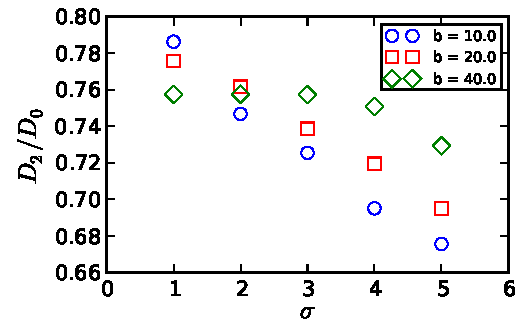
\includegraphics{dts_D2}
\caption{The transient diffusion coefficient for quantum spreading in
a banded sparse network. The ratio $D/D_0$ between the numerical diffusion 
coefficient and the expected value decreases as $\sigma$ increases. The effect
is stronger for low bandwidth.}
\end{figure}


Our first question was whether our rate equation analysis might
hold also for the quantum case, because in first order perturbation theory,
the transition probability $p_{nm}$ is proportional to $\left|\bra n|\mathcal{H} | m \ket\right|^2$.
Naively using our previously obtained suppression factor $g_s = \frac{D_{ERH}}{D_{\textrm{linear}}}$,
did not prove to be sufficient, as can be seen in \autoref{fig:d_vs_g}.

\begin{figure}
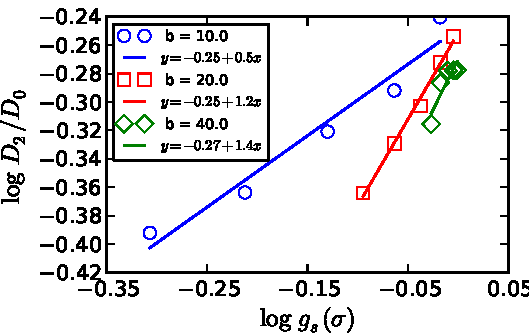
\includegraphics{dts_D2_vs_gs_loglog}
\caption{Scaled $D$ vs $g_s$. }\label{fig:d_vs_g}
\end{figure}
